% questions.tex —— 2022 年·新高考Ⅱ卷 · 题目内容片段（无答案）
% 由 tools/generate_projects.py 依来源总账自 2022/2022_数学真题_新高考Ⅱ_试题.md 生成，勿手改（改源 MD 后重跑）


\begin{gknotice}
\textbf{结构提示}：本卷为 \textbf{22 题制}。2024 年起新高考Ⅱ卷改为 19 题制，故本卷宜按知识点抽题使用，不宜整套限时模拟。

\textbf{适用省份}：海南、辽宁、重庆

\textbf{来源说明}：试题原文取自 deekur/gaokaomath（commit \texttt{34c13a6}，CC BY 4.0）之 \texttt{2022新高考2} PDF；本库配套解析为编者独立推导，\textbf{非官方标准答案}。
\end{gknotice}

\par\medskip

\gkpart{一、单选题}

\begin{gktip}
本题共 8 小题，每小题 5 分，共 40 分。在每小题给出的四个选项中，只有一项是符合题目要求的。
\end{gktip}

\begin{question}
\gkti{1}已知集合 $A=\{-1,1,2,4\}$，$B=\{x\mid|x-1|\le1\}$，则 $A\cap B=$（　　）

\begin{gkopts}(4)
\task A．$\{-1,2\}$
\task B．$\{1,2\}$
\task C．$\{1,4\}$
\task D．$\{-1,4\}$
\end{gkopts}

\end{question}
\begin{question}
\gkti{2}$(2+2\mathrm i)(1-2\mathrm i)=$（　　）

\begin{gkopts}(4)
\task A．$-2+4\mathrm i$
\task B．$-2-4\mathrm i$
\task C．$6+2\mathrm i$
\task D．$6-2\mathrm i$
\end{gkopts}

\Needspace{0.4\textheight}
\end{question}
\begin{question}
\gkti{3}图 1 是中国的古建筑中的举架结构，$AA'$，$BB'$，$CC'$，$DD'$ 是桁，相邻桁的水平距离称为步，垂直距离称为举。图 2 是某古建筑屋顶截面示意图，其中 $DD_1$，$CC_1$，$BB_1$，$AA_1$ 是举，$OD_1$，$DC_1$，$CB_1$，$BA_1$ 是相等的步，相邻桁的举步之比分别为 $\dfrac{DD_1}{OD_1}=0.5$，$\dfrac{CC_1}{DC_1}=k_1$，$\dfrac{BB_1}{CB_1}=k_2$，$\dfrac{AA_1}{BA_1}=k_3$。已知 $k_1$，$k_2$，$k_3$ 成公差为 $0.1$ 的等差数列，且直线 $OA$ 的斜率为 $0.725$，则 $k_3=$（　　）
\nopagebreak[4]
\begin{center}% 2022 新高考Ⅱ卷 3：中国古建筑「举架」结构（简化示意图）
% 原图为木构屋架写实线描，此处按简化示意重绘，不追求写实细节，只保留题意所需的阶梯关系：
% 底部大梁之上叠三层逐层收短的横梁，层间以瓜柱（短柱）支撑，梁端置桁（檩）。
% 相邻桁的水平距离（步）恒取 1，瓜柱高（举）自下而上取 0.5、0.7、0.8、0.9，
% 故屋面折线呈上陡下缓。右半侧自上而下标桁位 A'、B'、C'、D'，其正下方梁上对应点标 A、B、C、D，
% 竖直段 AA'、BB'、CC'、DD' 即「举」，相邻两点的水平间距即「步」。
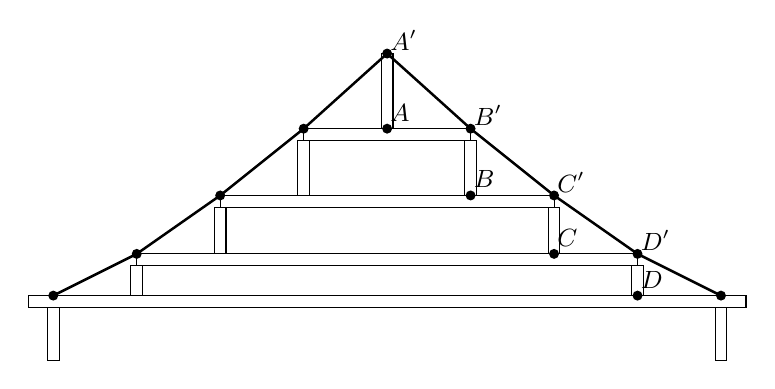
\begin{tikzpicture}[scale=1.06, font=\small]
  % ---- 梁：自下而上逐层收短（细长矩形示木料截面）----
  \draw (-4.3,-0.14) rectangle (4.3,0);
  \draw (-3,0.36)    rectangle (3,0.5);
  \draw (-2,1.06)    rectangle (2,1.2);
  \draw (-1,1.86)    rectangle (1,2.0);
  % ---- 檐柱（示意落地）----
  \draw (-4.07,-0.78) rectangle (-3.93,-0.14);
  \draw (3.93,-0.78)  rectangle (4.07,-0.14);
  % ---- 瓜柱：层间短柱，其高即「举」----
  \foreach \s in {-1,1}{
    \draw (3*\s-0.07,0)   rectangle (3*\s+0.07,0.36);
    \draw (2*\s-0.07,0.5) rectangle (2*\s+0.07,1.06);
    \draw (\s-0.07,1.2)   rectangle (\s+0.07,1.86);
  }
  \draw (-0.07,2.0) rectangle (0.07,2.9);          % 脊瓜柱
  % ---- 屋面折线：依次过各桁位 ----
  \draw[line width=0.9pt]
    (-4,0) -- (-3,0.5) -- (-2,1.2) -- (-1,2.0) -- (0,2.9)
           -- (1,2.0) -- (2,1.2) -- (3,0.5) -- (4,0);
  % ---- 桁位标记 ----
  \foreach \p in {(-4,0),(-3,0.5),(-2,1.2),(-1,2.0),(0,2.9),(1,2.0),(2,1.2),(3,0.5),(4,0)}
    { \fill \p circle (1.7pt); }
  \foreach \p in {(0,2.0),(1,1.2),(2,0.5),(3,0)} { \fill \p circle (1.7pt); }
  % ---- 标注（右半侧）----
  \node[above right, inner sep=1pt] at (0,2.9) {$A'$};
  \node[above right, inner sep=1pt] at (1,2.0) {$B'$};
  \node[above right, inner sep=1pt] at (2,1.2) {$C'$};
  \node[above right, inner sep=1pt] at (3,0.5) {$D'$};
  \node[above right, inner sep=1pt, yshift=1.5pt] at (0,2.0) {$A$};
  \node[above right, inner sep=1pt, yshift=1.5pt] at (1,1.2) {$B$};
  \node[above right, inner sep=1pt, yshift=1.5pt] at (2,0.5) {$C$};
  \node[above right, inner sep=1pt, yshift=1.5pt] at (3,0)   {$D$};
\end{tikzpicture}
\end{center}
\nopagebreak[4]
\nopagebreak[4]
\begin{center}% 2022 新高考Ⅱ卷 3：举架结构抽象出的屋顶截面折线图
% 左半支自原点 O 经 D、C、B 升至顶点 A，右半支关于过 A 的竖直线对称（不标字母）。
% 步长恒为 1，举依次取 0.5、0.7、0.8、0.9，即 O(0,0)、D(1,0.5)、C(2,1.2)、B(3,2.0)、A(4,2.9)。
% 虚线小阶梯给出各段的举与步：垂足 D_1(1,0)、C_1(2,0.5)、B_1(3,1.2)、A_1(4,2.0)，
% 水平段 OD_1、DC_1、CB_1、BA_1 四段等长（即「步」），竖直段 DD_1、CC_1、BB_1、AA_1 即「举」。
\begin{tikzpicture}[scale=1.12, font=\small]
  % ---- 坐标轴 ----
  \draw[-stealth] (-0.45,0) -- (8.95,0);
  \draw[-stealth] (0,-0.4) -- (0,3.45);
  % ---- 举步阶梯（虚线）----
  \draw[dashed] (0,0) -- (1,0) -- (1,0.5) -- (2,0.5) -- (2,1.2)
                     -- (3,1.2) -- (3,2.0) -- (4,2.0) -- (4,2.9);
  % ---- 屋顶截面折线 ----
  \draw[line width=0.9pt]
    (0,0) -- (1,0.5) -- (2,1.2) -- (3,2.0) -- (4,2.9)
          -- (5,2.0) -- (6,1.2) -- (7,0.5) -- (8,0);
  % ---- 点 ----
  \foreach \p in {(0,0),(1,0.5),(2,1.2),(3,2.0),(4,2.9),(1,0),(2,0.5),(3,1.2),(4,2.0)}
    { \fill \p circle (1.6pt); }
  % ---- 标注：折线点在左上，垂足在下/右 ----
  \node[below left,  inner sep=2pt] at (0,0)   {$O$};
  \node[above left,  inner sep=1pt] at (1,0.5) {$D$};
  \node[above left,  inner sep=1pt] at (2,1.2) {$C$};
  \node[above left,  inner sep=1pt] at (3,2.0) {$B$};
  \node[above,       inner sep=2pt] at (4,2.9) {$A$};
  \node[below,       inner sep=2pt] at (1,0)   {$D_1$};
  \node[below right, inner sep=1pt] at (2,0.5) {$C_1$};
  \node[below right, inner sep=1pt] at (3,1.2) {$B_1$};
  \node[below right, inner sep=1pt] at (4,2.0) {$A_1$};
\end{tikzpicture}
\end{center}
\nopagebreak[4]
\begin{gkopts}(4)
\task A．$0.75$
\task B．$0.8$
\task C．$0.85$
\task D．$0.9$
\end{gkopts}

\end{question}
\begin{question}
\gkti{4}已知向量 $\boldsymbol a=(3,4)$，$\boldsymbol b=(1,0)$，$\boldsymbol c=\boldsymbol a+t\boldsymbol b$，若 $\langle\boldsymbol a,\boldsymbol c\rangle=\langle\boldsymbol b,\boldsymbol c\rangle$，则 $t=$（　　）

\begin{gkopts}(4)
\task A．$-6$
\task B．$-5$
\task C．$5$
\task D．$6$
\end{gkopts}

\end{question}
\begin{question}
\gkti{5}甲、乙、丙、丁、戊 $5$ 名同学站成一排参加文艺汇演，若甲不站在两端，丙和丁相邻，则不同排列方式共有（　　）

\begin{gkopts}(4)
\task A．$12$ 种
\task B．$24$ 种
\task C．$36$ 种
\task D．$48$ 种
\end{gkopts}

\end{question}
\begin{question}
\gkti{6}若 $\sin(\alpha+\beta)+\cos(\alpha+\beta)=2\sqrt2\cos\left(\alpha+\dfrac\pi4\right)\sin\beta$，则（　　）

\begin{gkopts}(2)
\task A．$\tan(\alpha-\beta)=1$
\task B．$\tan(\alpha+\beta)=1$
\task C．$\tan(\alpha-\beta)=-1$
\task D．$\tan(\alpha+\beta)=-1$
\end{gkopts}

\end{question}
\begin{question}
\gkti{7}已知正三棱台的高为 $1$，上、下底面的边长分别为 $3\sqrt3$ 和 $4\sqrt3$，其顶点都在同一球面上，则该球的表面积为（　　）

\begin{gkopts}(4)
\task A．$100\pi$
\task B．$128\pi$
\task C．$144\pi$
\task D．$192\pi$
\end{gkopts}

\end{question}
\begin{question}
\gkti{8}已知函数 $f(x)$ 的定义域为 $\mathbf R$，且 $f(x+y)+f(x-y)=f(x)f(y)$，$f(1)=1$，则 $\displaystyle\sum_{k=1}^{22}f(k)=$（　　）

\begin{gkopts}(4)
\task A．$-3$
\task B．$-2$
\task C．$0$
\task D．$1$
\end{gkopts}

\par\medskip

\end{question}
\gkpart{二、多选题}

\begin{gktip}
本题共 4 小题，每小题 5 分，共 20 分。全部选对得 5 分，部分选对得 2 分，有选错得 0 分。
\end{gktip}

\begin{question}
\gkti{9}已知函数 $f(x)=\sin(2x+\varphi)\ (0<\varphi<\pi)$ 的图象关于点 $\left(\dfrac{2\pi}3,0\right)$ 中心对称，则（　　）

\begin{gkopts}(1)
\task A．$f(x)$ 在区间 $\left(0,\dfrac{5\pi}{12}\right)$ 单调递减
\task B．$f(x)$ 在区间 $\left(-\dfrac\pi{12},\dfrac{11\pi}{12}\right)$ 有两个极值点
\task C．直线 $x=\dfrac{7\pi}6$ 是曲线 $y=f(x)$ 的对称轴
\task D．直线 $y=\dfrac{\sqrt3}2-x$ 是曲线 $y=f(x)$ 的切线
\end{gkopts}

\end{question}
\begin{question}
\gkti{10}已知 $O$ 为坐标原点，过抛物线 $C:y^{2}=2px\ (p>0)$ 焦点 $F$ 的直线与 $C$ 交于 $A$，$B$ 两点，其中 $A$ 在第一象限，点 $M(p,0)$。若 $|AF|=|AM|$，则（　　）

\begin{gkopts}(2)
\task A．直线 $AB$ 的斜率为 $2\sqrt6$
\task B．$|OB|=|OF|$
\task C．$|AB|>4|OF|$
\task D．$\angle OAM+\angle OBM<180^\circ$
\end{gkopts}

\Needspace{0.4\textheight}
\end{question}
\begin{question}
\gkti{11}如图，四边形 $ABCD$ 为正方形，$ED\perp$ 平面 $ABCD$，$FB\parallel ED$，$AB=ED=2FB$。记三棱锥 $E\text{-}ACD$，$F\text{-}ABC$，$F\text{-}ACE$ 的体积分别为 $V_1$，$V_2$，$V_3$，则（　　）
\nopagebreak[4]
\begin{center}% 2022 新高考Ⅱ卷 11：正方形 ABCD 与同侧两条垂线 DE、BF
% 取 AB=2，立体坐标 A(0,0,0)、B(2,0,0)、C(2,2,0)、D(0,2,0)，DE⊥平面 ABCD 且 DE=2，
% BF⊥平面 ABCD 且 BF=1，即 E(0,2,2)、F(2,0,1)。
% 画布投影：(x,y,z) -> x·(1,0) + y·(0.42,0.30) + z·(0,1)。
% 虚线（被遮挡）：CD、DA、AC、DE；其余为可见实线。
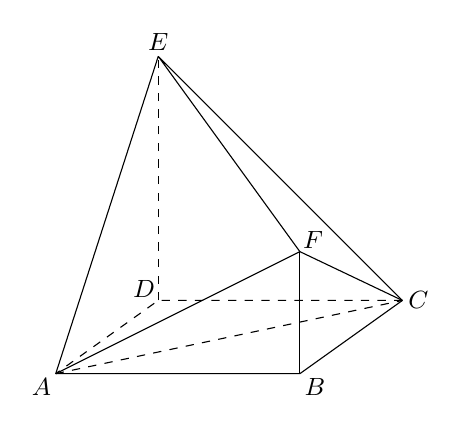
\begin{tikzpicture}[scale=1.55, font=\small]
  \coordinate (A) at (0,0);
  \coordinate (B) at (2,0);
  \coordinate (C) at (2.84,0.60);
  \coordinate (D) at (0.84,0.60);
  \coordinate (E) at (0.84,2.60);
  \coordinate (F) at (2,1.00);
  % 可见实线
  \draw (A) -- (B) -- (C);
  \draw (B) -- (F);
  \draw (E) -- (A)  (E) -- (C)  (E) -- (F);
  \draw (F) -- (A)  (F) -- (C);
  % 被遮挡
  \draw[dashed] (C) -- (D) -- (A);
  \draw[dashed] (A) -- (C);
  \draw[dashed] (D) -- (E);
  \node[below left,  inner sep=1.5pt] at (A) {$A$};
  \node[below right, inner sep=1.5pt] at (B) {$B$};
  \node[right,       inner sep=2pt]   at (C) {$C$};
  \node[above left,  inner sep=1pt]   at (D) {$D$};
  \node[above,       inner sep=2pt]   at (E) {$E$};
  \node[above right, inner sep=1pt]   at (F) {$F$};
\end{tikzpicture}
\end{center}
\nopagebreak[4]
\begin{gkopts}(4)
\task A．$V_3=2V_2$
\task B．$V_3=V_1$
\task C．$V_3=V_1+V_2$
\task D．$2V_3=3V_1$
\end{gkopts}

\end{question}
\begin{question}
\gkti{12}若 $x$，$y$ 满足 $x^{2}+y^{2}-xy=1$，则（　　）

\begin{gkopts}(2)
\task A．$x+y\le1$
\task B．$x+y\ge-2$
\task C．$x^{2}+y^{2}\le2$
\task D．$x^{2}+y^{2}\ge1$
\end{gkopts}

\par\medskip

\end{question}
\gkpart{三、填空题}

\begin{gktip}
本题共 4 小题，每小题 5 分，共 20 分。
\end{gktip}

\begin{question}
\gkti{13}已知随机变量 $X$ 服从正态分布 $N\left(2,\sigma^{2}\right)$，且 $P(2<X\le2.5)=0.36$，则 $P(X>2.5)=$ \gkblank{}．

\end{question}
\begin{question}
\gkti{14}曲线 $y=\ln|x|$ 经过坐标原点的两条切线的方程分别为 \gkblank{}，\gkblank{}．

\end{question}
\begin{question}
\gkti{15}设点 $A(-2,3)$，$B(0,a)$，若直线 $AB$ 关于 $y=a$ 对称的直线与圆 $(x+3)^{2}+(y+2)^{2}=1$ 有公共点，则 $a$ 的取值范围是 \gkblank{}．

\end{question}
\begin{question}
\gkti{16}已知直线 $l$ 与椭圆 $\dfrac{x^{2}}6+\dfrac{y^{2}}3=1$ 在第一象限交于 $A$，$B$ 两点，$l$ 与 $x$ 轴、$y$ 轴分别交于 $M$，$N$ 两点，且 $|MA|=|NB|$，$|MN|=2\sqrt3$，则 $l$ 的方程为 \gkblank{}．

\par\medskip

\end{question}
\gkpart{四、解答题}

\begin{gktip}
本题共 6 小题，共 70 分。解答应写出文字说明、证明过程或演算步骤。
\end{gktip}

\begin{question}
\gkti{17}\textbf{（10 分）} 已知 $\left\{a_n\right\}$ 是等差数列，$\left\{b_n\right\}$ 是公比为 $2$ 的等比数列，且 $a_2-b_2=a_3-b_3=b_4-a_4$。

  (1) 证明：$a_1=b_1$；

  (2) 求集合 $\left\{k\mid b_k=a_m+a_1,\ 1\le m\le500\right\}$ 中元素的个数。

\end{question}
\begin{question}
\gkti{18}\textbf{（12 分）} 记 $\triangle ABC$ 的内角 $A$，$B$，$C$ 的对边分别为 $a$，$b$，$c$，分别以 $a$，$b$，$c$ 为边长的三个正三角形的面积依次为 $S_1$，$S_2$，$S_3$。已知 $S_1-S_2+S_3=\dfrac{\sqrt3}2$，$\sin B=\dfrac13$。

  (1) 求 $\triangle ABC$ 的面积；

  (2) 若 $\sin A\sin C=\dfrac{\sqrt2}3$，求 $b$。

\Needspace{0.4\textheight}
\end{question}
\begin{question}
\gkti{19}\textbf{（12 分）} 在某地区进行流行病学调查，随机调查了 $100$ 位某种疾病患者的年龄，得到如下的样本数据的频率分布直方图。
\nopagebreak[4]
\begin{center}% 2022 新高考Ⅱ卷 19：年龄频率分布直方图
% 九组，组距均为 10（[0,10),…,[80,90)），频率/组距依次为
% 0.001、0.002、0.012、0.017、0.023、0.020、0.017、0.006、0.002（合计 ×10 = 1）。
% 纵轴刻度自下而上 0.001、0.002、0.006、0.012、0.017、0.020、0.023，各引水平虚线至对应矩形顶。
\begin{tikzpicture}[font=\small, x=0.088cm, y=260cm]
  % ---- 引至矩形顶的水平虚线 ----
  \draw[dashed] (0,0.001) -- (10,0.001);
  \draw[dashed] (0,0.002) -- (20,0.002);
  \draw[dashed] (0,0.006) -- (80,0.006);
  \draw[dashed] (0,0.012) -- (30,0.012);
  \draw[dashed] (0,0.017) -- (40,0.017);
  \draw[dashed] (0,0.020) -- (60,0.020);
  \draw[dashed] (0,0.023) -- (50,0.023);
  % ---- 直方图矩形 ----
  \draw ( 0,0) rectangle (10,0.001);
  \draw (10,0) rectangle (20,0.002);
  \draw (20,0) rectangle (30,0.012);
  \draw (30,0) rectangle (40,0.017);
  \draw (40,0) rectangle (50,0.023);
  \draw (50,0) rectangle (60,0.020);
  \draw (60,0) rectangle (70,0.017);
  \draw (70,0) rectangle (80,0.006);
  \draw (80,0) rectangle (90,0.002);
  % ---- 坐标轴 ----
  \draw[-stealth] (0,0) -- (97,0);
  \draw[-stealth] (0,0) -- (0,0.0258);
  % ---- 刻度 ----
  \foreach \x in {10,20,30,40,50,60,70,80,90}
    { \draw (\x,0) -- (\x,-0.00035); \node[below, inner sep=2pt] at (\x,-0.0002) {\footnotesize $\x$}; }
  \foreach \y/\lab in {0.001/0.001,0.002/0.002,0.006/0.006,0.012/0.012,0.017/0.017,0.020/0.020,0.023/0.023}
    { \draw (0,\y) -- (-1.6,\y); \node[left, inner sep=2pt] at (-1.6,\y) {\footnotesize $\lab$}; }
  \node[below left, inner sep=1.5pt] at (0,0) {$0$};
  % ---- 轴名 ----
  \node[right, inner sep=3pt] at (97,0) {年龄/岁};
  \node[above, inner sep=2.5pt] at (0,0.0258) {$\displaystyle\frac{\mbox{频率}}{\mbox{组距}}$};
\end{tikzpicture}
\end{center}
\nopagebreak[4]
  (1) 估计该地区这种疾病患者的平均年龄；（同一组中的数据用该区间的中点值为代表）

  (2) 估计该地区一位这种疾病患者的年龄位于区间 $[20,70)$ 的概率；

  (3) 已知该地区这种疾病患者的患病率为 $0.1\%$，该地区年龄位于区间 $[40,50)$ 的人口占该地区总人口的 $16\%$。从该地区中任选一人，若此人的年龄位于区间 $[40,50)$，求此人患这种疾病的概率。（以样本数据中患者的年龄位于各区间的频率作为患者的年龄位于该区间的概率，精确到 $0.0001$）

\Needspace{0.4\textheight}
\end{question}
\begin{question}
\gkti{20}\textbf{（12 分）} 如图，$PO$ 是三棱锥 $P\text{-}ABC$ 的高，$PA=PB$，$AB\perp AC$，$E$ 为 $PB$ 的中点。
\nopagebreak[4]
\begin{center}% 2022 新高考Ⅱ卷 20：三棱锥 P-ABC（PO⊥底面 ABC，E 为 PB 的中点）
% 立体坐标 A(0,0,0)、B(4√3,0,0)、C(0,12,0)、O(2√3,2,0)、P(2√3,2,3)、E(3√3,1,3/2)。
% 画布投影：(x,y,z) -> x·(1,0) + y·(-0.22,0.46) + z·(0,1)，故 C 落在左上远处、O 在底面内部、P 在 O 正上方。
% 深度方向取得较陡，是为了让汇于远点 C 的五条连线张开成可辨的扇形。
% 虚线（被遮挡）：PO（竖直）、CB、CO、CE；其余为可见实线。
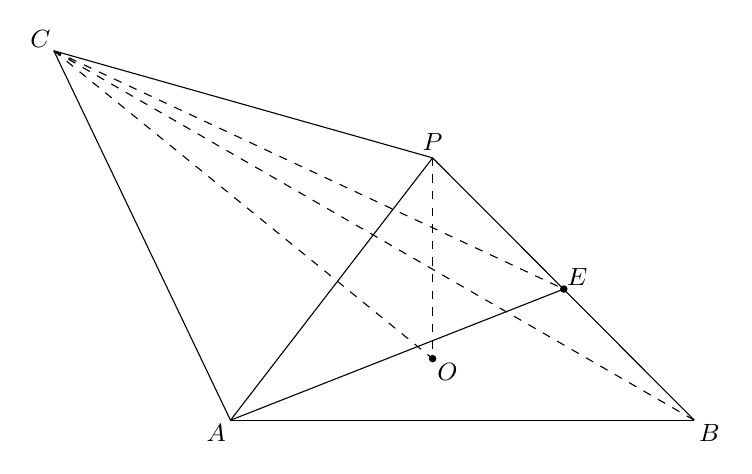
\begin{tikzpicture}[scale=0.85, font=\small]
  \coordinate (A) at (0,0);
  \coordinate (B) at (6.93,0);
  \coordinate (C) at (-2.64,5.52);
  \coordinate (O) at (3.02,0.92);
  \coordinate (P) at (3.02,3.92);
  \coordinate (E) at (4.98,1.96);
  % 可见实线
  \draw (A) -- (B);
  \draw (A) -- (C);
  \draw (P) -- (A)  (P) -- (B)  (P) -- (C);
  \draw (A) -- (E);
  % 被遮挡
  \draw[dashed] (P) -- (O);
  \draw[dashed] (C) -- (B)  (C) -- (O)  (C) -- (E);
  \fill (O) circle (1.6pt);
  \fill (E) circle (1.6pt);
  \node[below left,  inner sep=1.5pt] at (A) {$A$};
  \node[below right, inner sep=1.5pt] at (B) {$B$};
  \node[above left,  inner sep=1pt]   at (C) {$C$};
  \node[below right, inner sep=1.5pt] at (O) {$O$};
  \node[above,       inner sep=2.5pt] at (P) {$P$};
  \node[above right, inner sep=1pt]   at (E) {$E$};
\end{tikzpicture}
\end{center}
\nopagebreak[4]
  (1) 证明：$OE\parallel$ 平面 $PAC$；

  (2) 若 $\angle ABO=\angle CBO=30^\circ$，$PO=3$，$PA=5$，求二面角 $C\text{-}AE\text{-}B$ 正弦值。

\end{question}
\begin{question}
\gkti{21}\textbf{（12 分）} 已知双曲线 $C:\dfrac{x^{2}}{a^{2}}-\dfrac{y^{2}}{b^{2}}=1\ (a>0,\ b>0)$ 的右焦点为 $F(2,0)$，渐近线方程为 $y=\pm\sqrt3x$。

  (1) 求 $C$ 的方程；

  (2) 过 $F$ 的直线与 $C$ 的两条渐近线分别交于 $A$，$B$ 两点，点 $P\left(x_1,y_1\right)$，$Q\left(x_2,y_2\right)$ 在 $C$ 上，且 $x_1>x_2>0$，$y_1>0$。过 $P$ 且斜率为 $-\sqrt3$ 的直线与过 $Q$ 且斜率为 $\sqrt3$ 的直线交于点 $M$。从下面①②③中选取两个作为条件，证明另外一个成立。

  　① $M$ 在 $AB$ 上；② $PQ\parallel AB$；③ $|MA|=|MB|$。

\end{question}
\begin{question}
\gkti{22}\textbf{（12 分）} 已知函数 $f(x)=x\mathrm e^{ax}-\mathrm e^{x}$。

  (1) 当 $a=1$ 时，讨论 $f(x)$ 的单调性；

  (2) 当 $x>0$ 时，$f(x)<-1$，求 $a$ 的取值范围；

  (3) 设 $n\in\mathbf N^{*}$，证明：$\dfrac1{\sqrt{1^{2}+1}}+\dfrac1{\sqrt{2^{2}+2}}+\cdots+\dfrac1{\sqrt{n^{2}+n}}>\ln(n+1)$。

\par\medskip

\begin{gktip}
\textbf{试题来源}：deekur/gaokaomath（commit \texttt{34c13a6}，CC BY 4.0）之 \texttt{2022新高考2} PDF。
\end{gktip}

\end{question}